\section{Zastosowania grafów}

W dzisiejszych czasach grafy mają szerokie zastosowanie w wielu różnorodnych dziedzinach, takich jak informatyka, ekonomia, socjologia, chemia, lingwistyka, logistyka czy telekomunikacja. W tej sekcji przedstawię jedynie kilka przykładowych problemów oraz jak za pomocą teorii grafów mogą one zostać rozwiązane (nie wdając się w szczegóły algorytmów, które są ogólnodostępne \cites{cormen}{bondy}{banachowski}).


\subsection*{Mosty Królewieckie, cykl Eulera}

Jednym z pierwszych zastosowań teorii grafów było rozwiązanie zagadnienia mostów królewieckich. Problem został rozwiązany przez Leonarda Eulera w XVIII wieku \cite[48]{wilson}. 

Przez Królewiec przepływała rzeka Pregoła, w której rozwidleniach znajdowały się dwie wyspy. Ponad rzeką wybudowano siedem mostów, tak jak jest to pokazane na rysunku \ref{fig:bridges-of-konigsberg}. Pytanie brzmiało: czy można przejść przez każdy most dokładnie jeden raz i powrócić do punktu wyjścia. 

Jest to równoważne z pytaniem, czy graf pokazany na rysunku \ref{fig:bridges-graph} posiada cykl Eulera (skąd pochodzi nazwa ów cyklu). 

\begin{figure}[H]
\centering
\begin{minipage}[b]{.45\textwidth}
  \centering
  \begin{figure}[H]
  \centering
  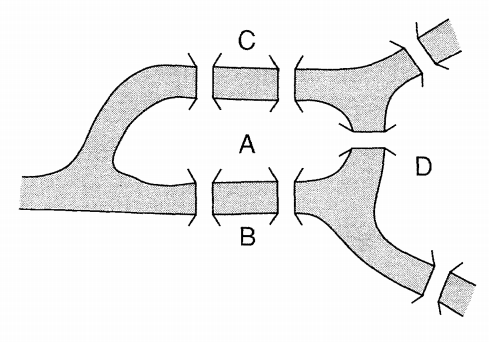
\includegraphics[width=\textwidth]{bridges-of-konigsberg.png}
  \end{figure}
\captionsetup{justification=centering}
\caption{Schemat mostów w~Królewcu z rzeką Pregołą \cite{wilson}}
\label{fig:bridges-of-konigsberg}
\end{minipage}
\begin{minipage}[b]{.45\textwidth}
  \centering
  \begin{tikzpicture}
\filldraw 
(0,2) node[label=left:A](1){}
(0,0.5) node[label=left:B](2){} 
(0,3.5) node[label=left:C](3){}
(3.5,2) node[label=right:D](4){}
(0,-0.5) node[color=white](5){};
\path[draw] (1)--(4);
\path[draw] (2)--(4);
\path[draw] (3)--(4);
\path
    (1) edge[bend left] (2)
    (2) edge[bend left](1)
    (1) edge[bend left] (3)
    (3) edge[bend left](1);
\end{tikzpicture}
\captionsetup{justification=centering}
\caption{Graf mostów w~Królewcu} \label{fig:bridges-graph}
\end{minipage}
\end{figure}


\subsection*{Zliczanie cząsteczek chemicznych}

Zliczanie cząsteczek chemicznych należy do jednych z najwcześniejszych przykładów użycia drzew. \cite[76]{wilson}. Wielki brytyjski matematyk Arthur Cayley był pierwszym, który dostrzegł związek pomiędzy wzorami strukturalnymi w chemii organicznej i grafami. \cite[59]{gutman}. Jako pierwszy wymyślił również określenie ,,drzewo'' \cite[60]{gutman}.

Cayley miał zamiar znaleźć sposób na obliczanie ile jest różnych izomerów \emph{alkanów}, których ogólny wzór sumaryczny ma postać $C_nH_{2n+2}$. Metodą budowania drzewa od jego centrum (centrów) udało mu się prawidłowo obliczyć ilość alkanów posiadających do jedenastu atomów węgla \cite[180]{aldous}. 

\begin{figure}[H]
\centering
\begin{minipage}[b]{.45\textwidth}
  \centering
\chemfig{C(-[:90]H)(-[:-90]H)(-[:0]H)(-[:180]C(-[:90]H)(-[:-90]H)(-[:180]C(-[:90]H)(-[:-90]H)(-[:180]C(-[:90]H)(-[:-90]H)(-[:180]H))))}
\captionsetup{justification=centering}
\caption{Wzór strukturalny $n$-butanu}
\label{fig:n-butane}
\end{minipage}
\begin{minipage}[b]{.45\textwidth}
  \centering
\chemfig{C(-[:-45,1.5]C(-[:-45]H)(-[:45]H)(-[:225]H))(-[:90]C(-[:90]H)(-[:0]H)(-[:180]H))(-[:-135,1.5]C(-[:-45]H)(-[:135]H)(-[:225]H))(-[:270]H)}
\captionsetup{justification=centering}
\caption{Wzór strukturalny 2-metylopropanu}
\end{minipage}
\end{figure}

Poniższa tabela przedstawia liczbę różnych alkanów $C_nH_{2n+2}$ posiadających $n$ atomów węgla, dla $n=1,\ldots,11$.

\begin{table}[H]
\begin{tabularx}{\textwidth}{rXXXXXXXXXXX}
\toprule
  $n$ & 1 & 2 & 3 & 4 & 5 & 6 & 7 & 8 & 9 & 10 & 11 \\ 
 liczba alkanów & 1 & 1 & 1 & 2 & 3 & 5 & 9 & 18 & 35 & 75 & 159 \\
 \bottomrule
\end{tabularx}
\end{table}

Rezultaty Cayleya wykorzystali i rozwinęli w swoich pracach inni, m.in. węgierski matematyk G. Pólya. W wyniku tych prac za pomocą metod teorii grafów zliczono wiele innych typów cząsteczek chemicznych.


\subsection*{Zagadnienie najkrótszej ścieżki}

Każdej krawędzi $e$ grafu $G$ możemy przypisać pewną nieujemną liczbę $w(e)$ (zwaną \textbf{wagą} tej krawędzi). Wówczas taki graf jest nazywany \textbf{grafem z wagami}. 

Grafy z wagami często występują w zastosowaniach teorii grafów \cite{bondy}. Na przykład, w grafach modelujących relację znajomości waga może wskazywać na to, jak dobrze dane osoby znają się, a w grafach modelujących sieć połączeń komunikacyjnych -- odległość pomiędzy dwoma punktami albo koszt wybudowania lub utrzymania takiego połączenia. 

Zadanie polega na znalezieniu ścieżki pomiędzy dwoma wybranymi punktami (lub ich większej ilości), której suma wag krawędzi jest najmniejsza. Do rozwiązania tego problemu może posłużyć algorytm Dijkstry działąjący w czasie $O(E\log(V))$. Dla grafów planarnych istnieje szybszy algorytm, który działa w czasie liniowym \cite{henzinger}. 

Warto zwrócić w tym miejscu uwagę, że również trasowanie w sieci Internet i wybór odpowiedniej drogi dla pakietów zawdzięczamy teorii grafów (np. protokół OSPF korzysta z algorytmu Dijkstry). 


\subsection*{Problem chińskiego listonosza}

W swojej pracy listonosz pobiera listy z poczty, dostarcza je, po czym wraca do budynku poczty. Musi przejść każdą ulicę przynajmniej jeden raz. Zadanie polega na znalezieniu najkrótszej drogi dla listonosza. Zagadnienie to jest znane pod nazwą \emph{problemu chińskiego listonosza}, ponieważ było po raz pierwszy rozpatrywane przez chińskiego matematyka Kuana (1962) \cite[62]{bondy}. 

Dla grafów eulerowskich problem sprowadza się do znalezienia cyklu Eulera (ponieważ taki cykl przechodzi przez każdą krawędź dokładnie raz). Problem ten możemy łatwo rozwiązać w takim przypadku, np. stosując algorytm Fleury'ego. 


\subsection*{Problem komiwojażera}

Podróżujący sprzedawca chce odwiedzić daną listę miast i powrócić do punktu początkowego. Mając dane czasy podróży pomiędzy miastami, w jaki sposób sprzedawca powinien zaplanować podróż, żeby odwiedzić wszystkie dokładnie raz w jak najkrótszym czasie? Zagadnienie to jest znane pod nazwą \emph{problemu komiwojażera} i jest równoważne ze znalezieniem takiego cyklu Hamiltona w danym grafie ważonym, w którym suma wag jest najmniejsza.

W przeciwieństwie do problemu chińskiego listonosza, nie jest znany efektywny\footnote{tj. działający w czasie wielomianowym} algorytm rozwiązujący problem komiwojażera. Dlatego często pożądane jest znalezienie odpowiednio dobrego (ale niekoniecznie najlepszego) rozwiązania \cite[65]{bondy}. 


\subsection*{Problem najkrótszych połączeń}

Pomiędzy miastami ma być wybudowana sieć połączeń kolejowych. Dane są koszty $c_{ij}$ wybudowania połączenia pomiędzy miastami $v_i$ i $v_j$. Zadanie polega na zaprojektowaniu sieci połączeń tak, aby zminimalizować koszt konstrukcji całej sieci. 

Problem sprowadza się do obliczenia minimalnego drzewa rozpinającego na danym grafie, co możemy uzyskać stosując np. algorytm Kruskala.


\subsection*{Problem stworzenia niezawodnej sieci komunikacyjnej}

Graf może reprezentować sieć komunikacyjną, którego wierzchołki to stacje komunikacyjne (lub którego krawędzie to połączenia komunikacyjne). Jaka jest minimalna liczba $k$ stacji (lub połączeń), których awaria zaburzy komunikację w tej sieci (tj. rozspójni graf). Im większa ta liczba tym bardziej niezawodna jest sieć. 

Dla $k=1$ problem redukuje się do problemu najkrótszych połączeń. Dla $k>1$ problem jest nierozwiązany i jest uważany za trudny (jednak dla grafów pełnych istnieje proste rozwiązanie) \cite[48]{bondy}. 


\subsection*{Problem przydziału personelu}

W pewnej firmie $n$ pracowników $X_1,X_2,\ldots,X_n$ jest dostępnych do wykonania $n$ zadań $Y_1,Y_2,\ldots,Y_n$. Każdy pracownik jest wykwalifikowany do wykonania jednego lub więcej z tych zadań. Czy można przypisać każdego pracownika do jednego zadania, do którego jest wykwalifikowany? 

Możemy utworzyć graf dwudzielny $G$ z podziałem wierzchołków na rozłączne zbiory $X$ i $Y$, gdzie $X=\{x_1,x_2,\ldots,x_n\}$ oraz $Y=\{y_1,y_2,\ldots,y_n\}$, w którym wierzchołek $x_i$ jest połączony krawędzią z wierzchołkiem $y_i$, gdy pracownik $X_i$ jest zdolny wykonać zadanie $Y_j$. Problem sprowadza się do sprawdzenia czy dany graf $G$ posiada skojarzenie doskonałe (co możemy stwierdzić na mocy twierdzenia \ref{theorem:hall}).


\subsection*{Problem rozkładu zadań}

W szkole jest $m$ nauczycieli $X_1,X_2,\ldots,X_m$ oraz $n$ klas $Y_1,Y_2,\ldots,Y_n$. Każdy nauczyciel $X_i$ powinien uczyć klasę $Y_j$ przez $p_{ij}$ godzin lekcyjnych. Zadanie polega na takim rozplanowaniu harmonogramu zajęć, aby zajęcia skończyły się jak najwcześniej. 

Możemy utworzyć graf dwudzielny $G$ z podziałem wierzchołków na rozłączne zbiory $X$ i $Y$, gdzie $X=\{x_1,x_2,\ldots,x_m\}$ oraz $Y=\{y_1,y_2,\ldots,y_n\}$, w którym wierzchołek $x_i$ jest połączony $p_{ij}$ krawędziami z wierzchołkiem $y_i$. W danym momencie nauczyciel może uczyć co najwyżej jedną klasę oraz dana klasa może być uczona przez co najwyżej jednego nauczyciela. 

Problem rozkładu zadań można rozwiązać stosując kolorowanie krawędzi -- indeks chromatyczny odpowiada minimalnej sumarycznej liczbie godzin lekcyjnych, po których wszystkie klasy odbędą wymaganą ilość poszczególnych godzin lekcyjnych. W grafie dwudzielnym indeks chromatyczny jest równy maksymalnemu stopniowi wierzchołka \cite[93]{bondy}.


\subsection*{Problem magazynowania}

Firma produkuje $n$ chemikaliów $C_1,C_2\ldots,C_n$. Pewne pary tych chemikaliów nie są kompatybilne i mogą powodować eksplozje w przypadku kontaktu. Jako środek zapobiegawczy firma chce zrobić podzielić magazyny na przedziały i trzymać niekompatybilne chemikalia w osobnych przedziałach. Jaka jest minimalna liczba przedziałów, które powinny być utworzone?

Możemy utworzyć graf $G$ ze zbiorem wierzchołków $\{v_1,v_2,\ldots,v_n\}$, w którym dwa wierzchołki $v_i$ oraz $v_j$ są połączone krawędzią, gdy chemikalia $C_i$~oraz $C_j$ nie są kompatybilne. Wówczas łatwo zauważyć, że minimalna liczba przedziałów, którą należy utworzyć jest równa liczbie chromatycznej grafu $G$. 


\subsection*{Telekomunikacja}

W sieci komórkowej obszar podzielony jest na komórki w sposób, który zależy od  ukształtowania terenu, zabudowań oraz innych czynników mających wpływ na siłę i jakość odbieranego sygnału. Komórki te mają w przybliżeniu kształt sześciokątów, kwadratów lub okręgów, ale umownie przedstawiane są w postaci sześciokątów. W każdej komórce jest stacja bazowa, do której przypisany jest zakres używanych częstotliwości. Częstotliwości mogą być używane ponownie w innych komórkach pod warunkiem, że ta sama częstotliwość nie jest używana przez dwie sąsiadujące ze sobą komórki (ponieważ to mogłoby powodować zakłócenia sygnału -- tzw. \emph{przesłuch}).

W jaki sposób podzielić dostępne częstotliwości, aby spełniony był powyższy warunek? Problem ten możemy sprowadzić do zagadnienia kolorowania wierzchołków, co zostało przedstawione na rysunku \ref{fig:gsm} (inny kolor, oznacza inny zakres częstotliwości). Okazuje się, że cały zakres częstotliwości możemy podzielić na trzy rozłączne podzbiory, aby móc zgodnie z założeniem efektywnie pokryć cały obszar. 

\begin{figure}[H]
\caption{Schemat komórek w sieci GSM \cite{dharwadker}}\label{fig:gsm}
\centering
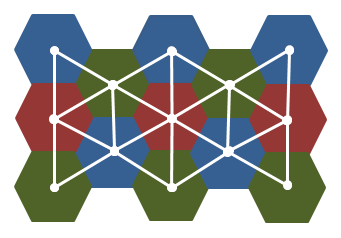
\includegraphics[width=0.6\textwidth]{gsm.png}
\end{figure}


\subsection*{Planarność}

Istnieje wiele praktycznych sytuacji, w których ważne jest stwierdzenie czy dany graf jest planarny i jeśli tak, to jak wygląda jego rysunek płaski. Na przykład, dana jest płytka elektroniczna, na której mają być wydrukowane przewody. Czy istnieje taki sposób ich rozmieszczenia, by połączenia nie przecinały się?

Problem ten możemy rozwiązać stosując algorytm skonstruowany przez Demoucrona, Malgrange'a i Pertuiseta (1964) \cite[163]{bondy}.


\subsection*{Inne zastosowania}

Ponadto grafy znalazły zastosowanie w wielu innych dziedzinach, takich jak:

\begin{itemize}
\setlength\itemsep{0em}
\item systemy rekomendacji,
\item wykrywanie oszustw,
\item wykrywanie spamu,
\item ranking stron w wyszukiwarce,
\item drzewa przeszukiwań binarnych,
\item bazy danych (B-drzewa),
\item sieci przepływowe,
\item sieci znajomych.
\end{itemize}
